% -------------------------------------------------------------------------------- %
% Latex file: `target-image.tex`
% Description:
% Speaking about cropped image cameramen details
% -------------------------------------------------------------------------------- %

% -------------------------------------------------------------------------------- %
\begin{frame}
    \frametitle{Selected Deep Nets Compression Techniques}
        % \centering \Huge
        \begin{center}
            {\fontsize{40}{50}\selectfont \emph{Input Dataset}}
        \end{center}
        \begin{center}
            \emph{Describing selected Input Target Image for our trials}
        \end{center}
\end{frame}

% Identifyed Target Image for Training Siren Models
% -------------------------------------------------------------------------------- %
\begin{frame}
    \frametitle{Identifyed Target Image for Training Siren Models}
        We decide to adopt, as in Siren related paper, Camera image as our target image of which we aim at inferring an implicit representation to be
        compared against to jpeg compressed couterpart images as well as pruned, quantized and both pruned-quantized compressed models


        \begin{columns}
            \column{0.5\textwidth}
            \begin{figure}
            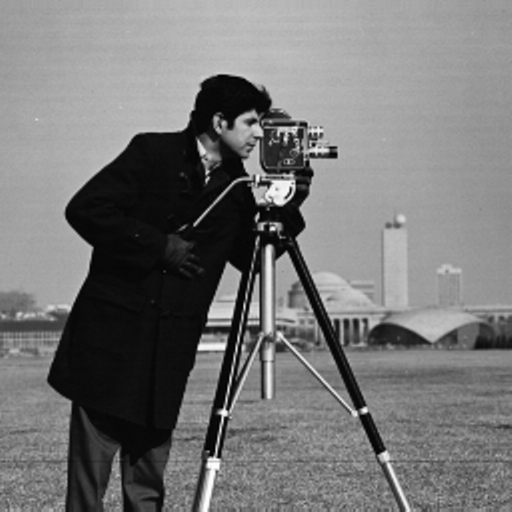
\includegraphics[scale=0.2]{slides/experiments/target-image/images/cameramen_512x512.png}
            \caption{Camera 512x521 target image}
            \end{figure}

        \column{0.5\textwidth}
            \begin{table}
            \begin{tabular}{ll}
            \hline
                    Image Feature & Value \\
            \hline
                name &      Camera \\
                shape &  (512, 512) \\
            size\_byte &      262144 \\
            image\_band &        (L,) \\
            \hline
            \end{tabular}
            \caption{Camera Image Characteristics }
            \end{table}

            \end{columns}
            Camera Image, which is a picture where a man was shoted while he was recoding via camera located on a top of tripod.
\end{frame}
